\documentclass[10pt,twocolumn]{article}

\usepackage[a4paper,margin=0.70in]{geometry}
\usepackage{graphicx}
\usepackage{booktabs}
\usepackage{array}
\usepackage{hyperref}
\usepackage{xcolor}
\usepackage{caption}
\usepackage{subcaption}
\usepackage{amsmath}
\usepackage{microtype}
\usepackage{enumitem}
\usepackage{float}
\usepackage{url}

\hypersetup{
  colorlinks=true,
  linkcolor=blue!55!black,
  citecolor=blue!55!black,
  urlcolor=blue!55!black
}

\setlist[itemize]{leftmargin=1.15em,itemsep=1pt,topsep=2pt}
\captionsetup{font=small,labelfont=bf}
\setlength{\columnsep}{0.24in}
\emergencystretch=1.5em
\Urlmuskip=0mu plus 2mu\relax

\newcommand{\githuburl}{\textbf{To be replaced after public GitHub upload}}
\newcommand{\weightsurl}{\textbf{To be replaced after model-weight upload}}

\title{\vspace{-0.55in}\textbf{LeRobot ACT Policy Generalization on CALVIN ABC$\rightarrow$D}}
\author{
  Assignment Report\\
  GitHub Repository: \githuburl\\
  Model Weights: \weightsurl
}
\date{June 26, 2026}

\begin{document}
\maketitle
\sloppy

\begin{abstract}
This report studies cross-environment generalization for Action Chunking with Transformers (ACT) using the LeRobot policy stack on the CALVIN ABC$\rightarrow$D benchmark. Two policies are trained with the same ACT architecture and hyperparameters: an A-only policy trained only on environment A and an ABC-joint policy trained on mixed A, B, and C data. Both are evaluated zero-shot in unseen environment D using offline action L1 error and closed-loop CALVIN rollouts. The final implementation uses two RGB camera views, robot state, official CALVIN language embeddings, action chunk size 10, temporal ensembling, and an effective stop at 88k training steps. The A-only model obtains 0.136686 D offline action L1, 22\% D SR@1, and 0.32 average completed subtasks. The ABC-joint model obtains 0.114896 D offline action L1, 38\% D SR@1, and 0.56 average completed subtasks. The main finding is narrow but consistent: under the same ACT design, mixing A/B/C training data improves zero-shot transfer to the held-out visual distribution D.
\end{abstract}

\section{Introduction}

Robotic imitation learning is easy to evaluate on the scene where demonstrations were collected, but much harder to trust after the visual environment changes. Background color, camera viewpoint, object placement, and small appearance details can change the visual features used by a policy even when the intended manipulation skill is the same. This issue is central to embodied AI: a robot policy should learn a task-relevant mapping from observation and goal to action, rather than memorizing one tabletop scene.

The assignment asks for a compact ACT-based study on CALVIN \cite{mees2022calvin}. CALVIN is a language-conditioned long-horizon manipulation benchmark with several related but visually distinct simulated environments. In the ABC$\rightarrow$D protocol, environments A, B, and C are available for training, while D is held out for zero-shot evaluation. This report follows that protocol with two final formal policies. The first policy is trained only on A. The second policy is trained on A, B, and C jointly. The architecture, optimizer, loss, input resolution, action chunk length, language-conditioning mechanism, evaluation scripts, and stopping rule are fixed between the two runs.

ACT, introduced by Zhao et al. \cite{zhao2023act}, predicts a short chunk of future actions instead of a single action. This design reduces the effective decision horizon and can make fine manipulation smoother. The same property also creates a failure mode under visual shift: if the first observation is interpreted incorrectly, a whole chunk can be biased in the wrong direction. The experiment is therefore designed around one practical question: does the broader visual support of A/B/C training make ACT more robust when it is rolled out in unseen D?

The answer in this workspace is yes, with a clear but not exaggerated margin. A-only fits its own training environment better, reaching lower in-domain validation L1. However, ABC-joint obtains lower held-out D action error and higher closed-loop D success. This distinction is important for reporting: training-validation loss alone is not a sufficient proxy for cross-environment deployment quality.

\section{Related Work}

\paragraph{Language-conditioned manipulation benchmarks.}
CALVIN, short for Composing Actions from Language and Vision, was proposed as a benchmark for long-horizon language-conditioned robot manipulation \cite{mees2022calvin}. Its goal is to evaluate policies that map visual observations and natural-language goals to long sequences of actions. The benchmark emphasizes zero-shot generalization to novel instructions and novel environments. The official CALVIN repository and dataset release provide the simulation environment, dataset splits, and task oracle used by this report \cite{calvinrepo}.

\paragraph{Action chunking for imitation learning.}
ACT was introduced in the ALOHA work on low-cost bimanual manipulation \cite{zhao2023act}. Its key idea is to predict action chunks with a Transformer policy and a variational training objective. In the original setting, chunking helped reduce compounding error by shortening the effective horizon of autoregressive control. LeRobot exposes ACT as a lightweight policy for imitation learning and recommends it as a practical starting point because it trains quickly and has modest compute requirements \cite{lerobotact}. This assignment uses that LeRobot ACT implementation rather than replacing it with a larger policy class.

\paragraph{LeRobot tooling and dataset format.}
LeRobot is an open-source robotics learning stack from Hugging Face that provides policy implementations, dataset tooling, and training/evaluation utilities \cite{lerobotrepo,lerobotact}. The local data used here is a parquet conversion of CALVIN into a LeRobot-compatible format \cite{fywangdataset}. The conversion is useful because it lets the experiment reuse existing Python, PyArrow, and LeRobot-style loading tools while preserving the CALVIN ABC$\rightarrow$D split semantics.

\section{Dataset and Environment}

\subsection{Split Definition}

The final protocol uses the CALVIN ABC$\rightarrow$D split. Training data comes from environments A, B, and C. Zero-shot evaluation uses environment D only. The A-only policy sees only A during training and training-validation. The ABC-joint policy sees a mixture of A, B, and C during training and training-validation. D is not used for model selection during training; it is evaluated after the best 88k checkpoint is selected from the training-environment validation metric.

\begin{table}[H]
\centering
\caption{Local CALVIN episode coverage used by the final protocol.}
\label{tab:data}
\resizebox{\linewidth}{!}{%
\begin{tabular}{llr}
\toprule
Environment & Role & Episodes \\
\midrule
A & A-only and ABC-joint train & 6089 \\
B & ABC-joint train & 6115 \\
C & ABC-joint train & 5666 \\
D & zero-shot evaluation & 1087 \\
\bottomrule
\end{tabular}
}
\end{table}

\subsection{Observation and Action Contract}

The policy input contains two RGB views and a state vector. The static camera captures the tabletop scene; the gripper camera captures wrist-centric visual detail. Robot proprioception contributes 15 state dimensions. The language goal is represented by the official 384D CALVIN SBERT embedding associated with the task annotation. The embedding is concatenated with proprioception, so the effective state dimension is 399.

The action target is the 7D CALVIN relative action: six dimensions for end-effector motion and one gripper command. A training example at time \(t\) supervises a future action chunk \(a_{t:t+K-1}\). When a chunk reaches beyond the end of an episode, padding masks remove invalid positions from the reconstruction loss. This is important because otherwise short terminal windows would bias the loss toward padded values.

\subsection{Closed-loop Runtime}

Closed-loop evaluation uses the official CALVIN PyBullet environment and task oracle. The rollout script loads a LeRobot checkpoint, converts CALVIN observations into the policy input format, decodes an action, and sends that action back to the environment. No scripted planner, oracle executor, or replay fallback is used to execute robot actions. The metric therefore reflects the learned ACT policy path.

\begin{figure}[H]
\centering
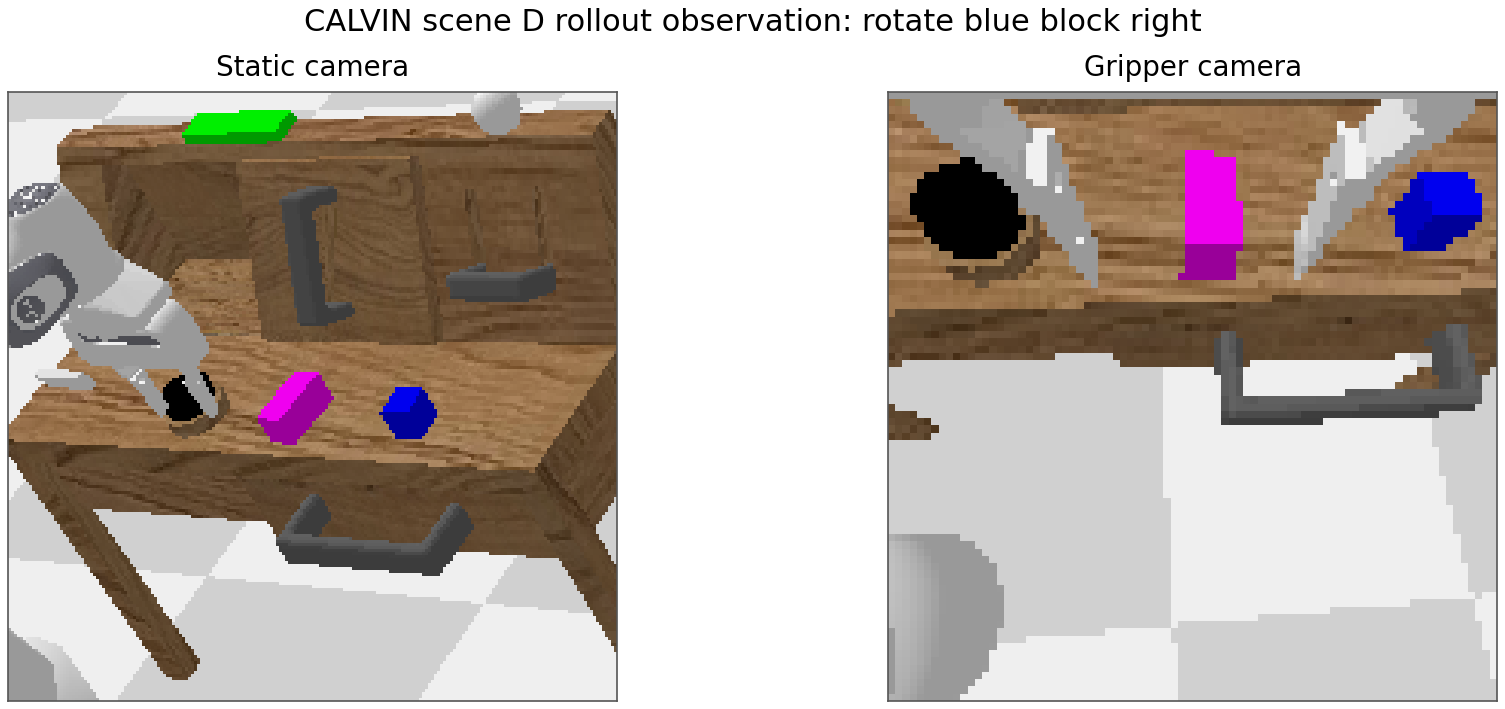
\includegraphics[width=\linewidth]{figures/formal_protocol/calvin_scene_d_rollout_snapshot.png}
\caption{Example observation from the official CALVIN scene-D rollout environment used for zero-shot testing. The left panel shows the static camera and the right panel shows the gripper camera for the task annotation ``take the blue block and rotate it to the right.''}
\label{fig:scene_d_snapshot}
\end{figure}

\section{Method}

\subsection{ACT Objective}

ACT predicts a block of future actions from the current observation:
\[
  \hat{a}_{t:t+K-1} = \pi_{\theta}(o_t, z),
\]
where \(z\) is the latent variable used by the ACT variational objective. During training, the encoder observes the target action sequence and infers a posterior over \(z\). The decoder reconstructs the action chunk conditioned on image features, state features, and the latent variable. The objective is:
\begin{equation}
\mathcal{L} = \mathcal{L}_{\mathrm{L1}} + \lambda_{\mathrm{KL}}\mathcal{L}_{\mathrm{KL}},
\end{equation}
where \(\mathcal{L}_{\mathrm{L1}}\) is the masked action reconstruction loss and \(\mathcal{L}_{\mathrm{KL}}\) regularizes the latent posterior toward a unit Gaussian. The final runs use \(\lambda_{\mathrm{KL}}=10\).

\subsection{Language-conditioned State Construction}

CALVIN tasks are goal-conditioned. A visually similar initial state can require different next actions depending on whether the instruction is, for example, to move a slider, open a drawer, or switch on a light. The final implementation therefore adds language conditioning while keeping the ACT network simple. The official CALVIN SBERT embedding is appended to the robot state before it is passed to LeRobot ACT. This is a small architectural change: the action decoder, chunking mechanism, optimizer, and loss remain ACT.

\subsection{Chunk Length and Temporal Ensemble}

The final chunk size is 10. A longer chunk can produce smoother behavior, but it can also carry a wrong visual interpretation for too many control steps. A short chunk increases the frequency at which the policy can correct from a new observation. Temporal ensembling is used with coefficient 0.01 to combine overlapping chunk predictions. In this report it is treated as an inference stabilizer, not as a separate controller.

\section{Experimental Protocol}

\subsection{Training Runs}

Both formal runs were trained to an effective stop at step 88000. The command cap was 100000 steps, but training was intentionally stopped after the step-88000 validation pass and the best checkpoint at step 88000 was used for evaluation. Both policies use the same architecture and hyperparameters; only the training environment list differs.

\begin{table*}[t]
\centering
\caption{Shared hyperparameters and implementation settings for the final ACT policies.}
\label{tab:hparams}
\begin{tabular}{llll}
\toprule
Category & Setting & Value & Notes \\
\midrule
Data & Format & HF parquet & LeRobot-style CALVIN conversion \\
Data & Train environments & A or A,B,C & only difference between runs \\
Input & Camera views & static, gripper & RGB images resized to 224 \\
Input & State dimension & 399 & 15 robot + 384 language \\
Action & Action dimension & 7 & relative pose + gripper \\
ACT & Chunk size & 10 & masked near episode end \\
ACT & Transformer width & 512 & shared across runs \\
ACT & Attention heads & 8 & shared across runs \\
ACT & Encoder / decoder layers & 4 / 1 & LeRobot ACTPolicy \\
ACT & Feed-forward dimension & 3200 & shared across runs \\
Optimization & Optimizer & AdamW & weight decay 1e-4 \\
Optimization & Learning rate & 1e-5 & same for both runs \\
Optimization & Batch size & 128 & final continuation runs \\
Loss & Objective & Action L1 + KL & KL weight 10 \\
Logging & Tracking & W\&B offline + CSV & curves exported locally \\
Stopping & Effective step & 88000 & best checkpoint at step 88000 \\
\bottomrule
\end{tabular}
\end{table*}

\subsection{Offline Evaluation}

Offline evaluation computes action reconstruction loss on the held-out D validation split. It does not interact with the simulator, so it is not a success-rate metric. Its value is still useful because it checks whether the policy predicts actions closer to D demonstrations when conditioned on D observations and language goals.

\subsection{Closed-loop Evaluation}

Closed-loop evaluation runs 50 CALVIN task chains in scene D. The main metric in this report is SR@1, the fraction of chains in which the first subtask is completed. Average completed subtasks is also reported because CALVIN chains are long-horizon. The metric is stricter than offline loss because the model must recover from its own states after each action.

\section{Results}

\begin{figure*}[t]
\centering
\begin{subfigure}{0.49\textwidth}
\centering
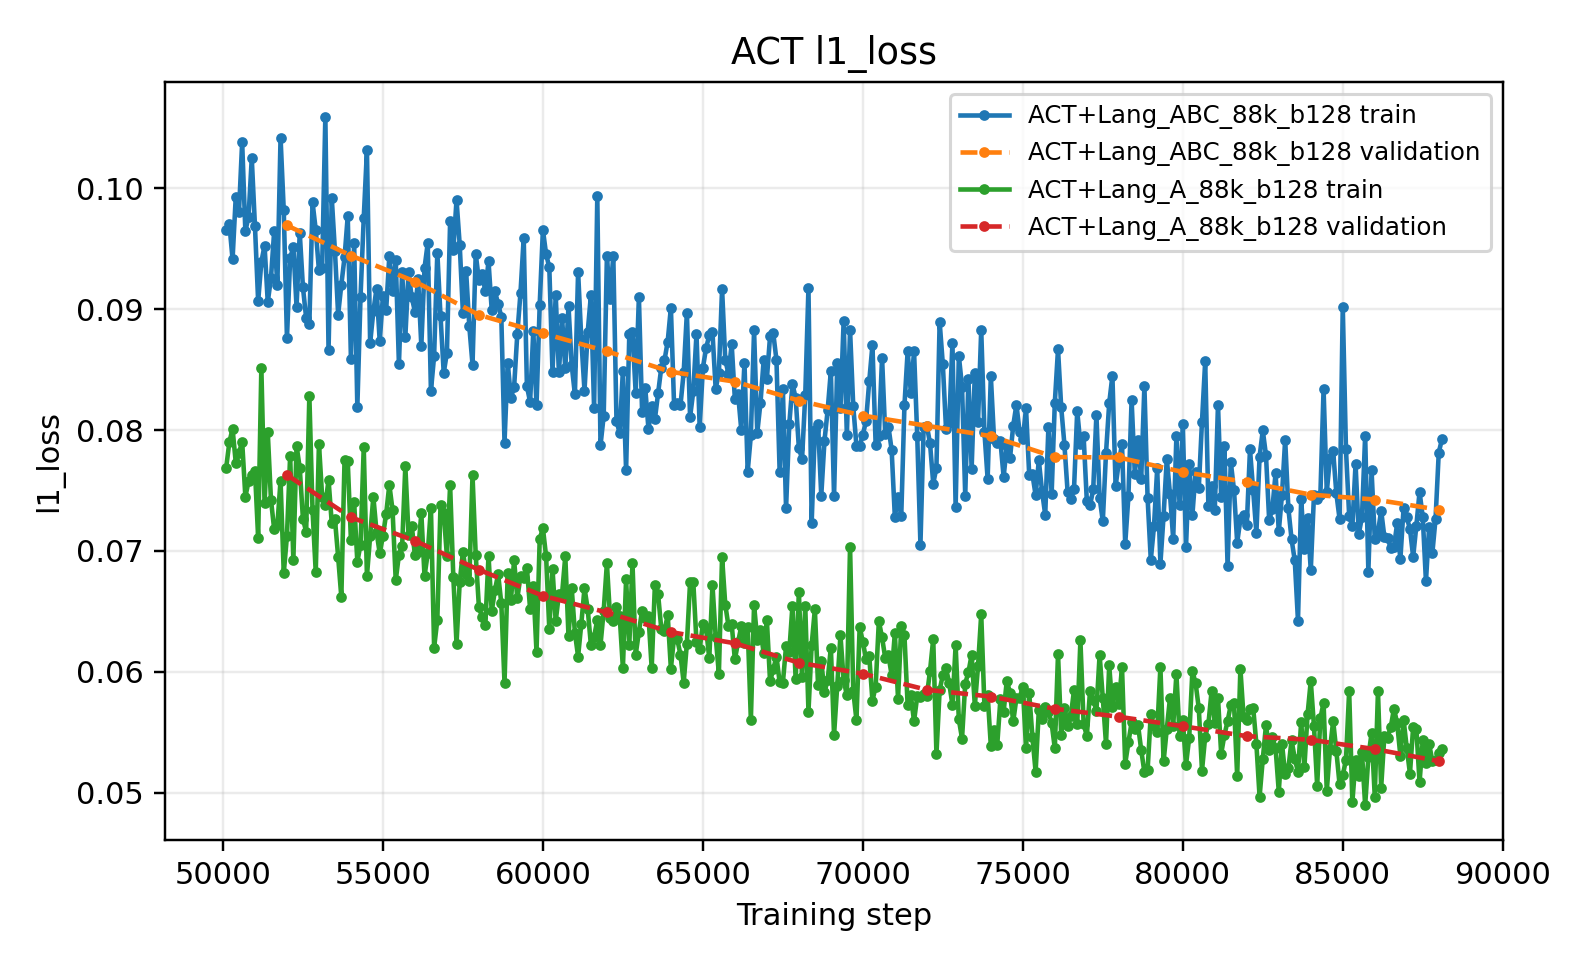
\includegraphics[width=\linewidth]{figures/formal_protocol/l1_loss.png}
\caption{Action L1 loss.}
\label{fig:l1}
\end{subfigure}
\hfill
\begin{subfigure}{0.49\textwidth}
\centering
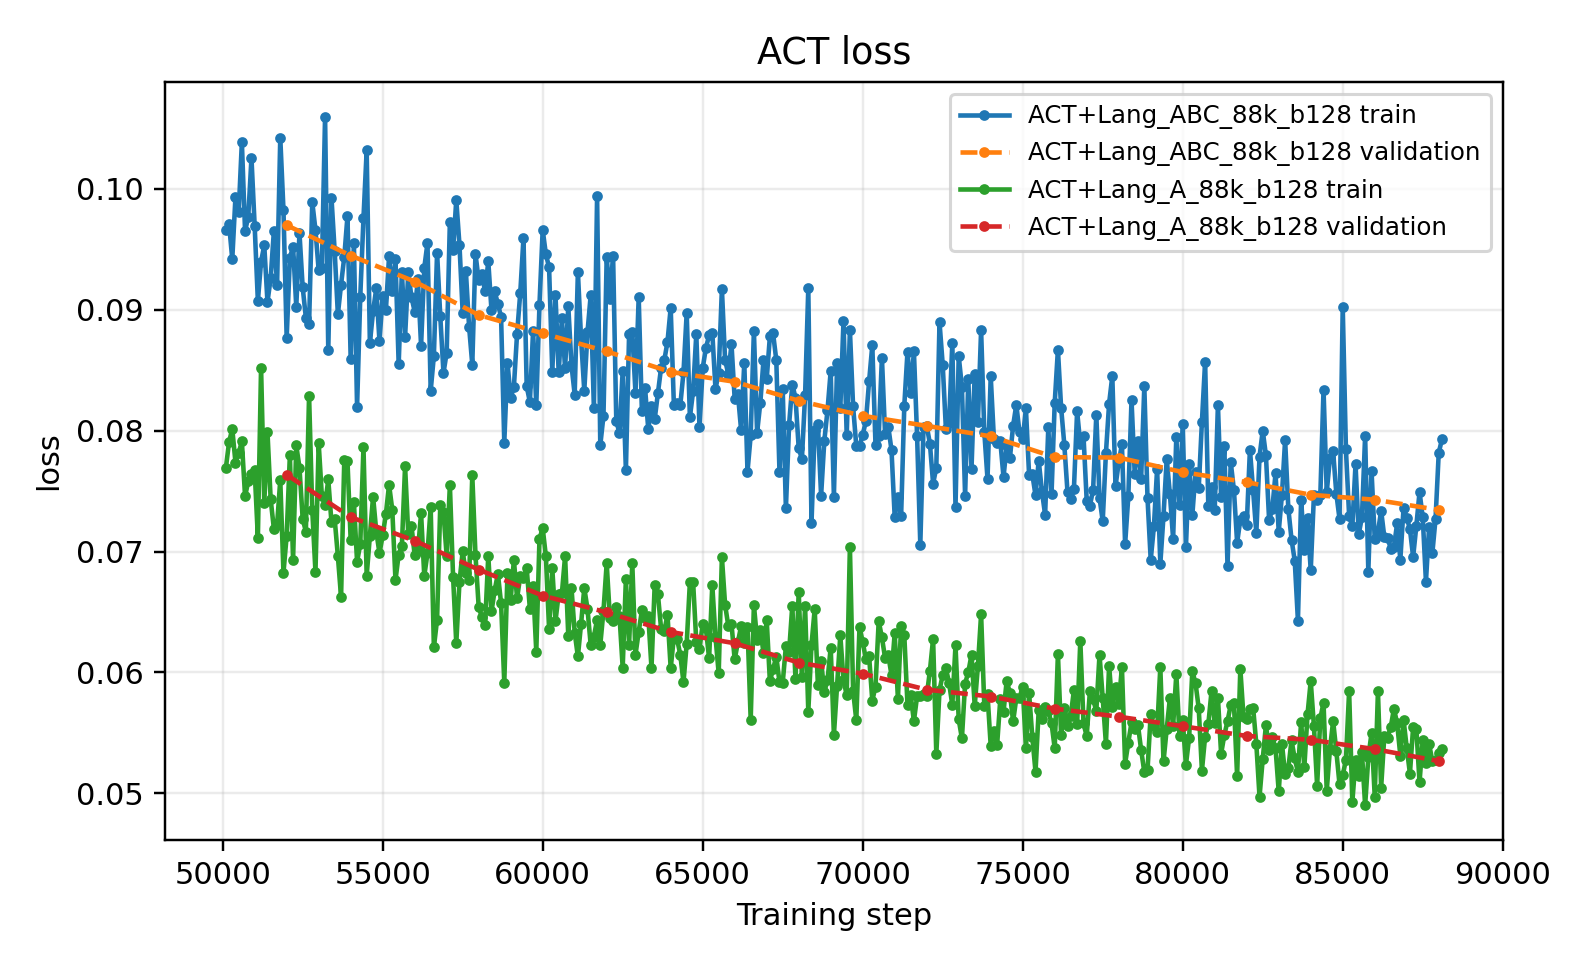
\includegraphics[width=\linewidth]{figures/formal_protocol/loss.png}
\caption{Total ACT loss.}
\label{fig:loss}
\end{subfigure}
\caption{Training curves exported from W\&B-compatible offline logs and local \texttt{metrics.csv} files. Solid lines are training metrics and dashed lines are validation metrics.}
\label{fig:curves}
\end{figure*}

\subsection{Training Convergence}

Figure~\ref{fig:curves} shows the final continuation segment. The A-only model reaches lower training-environment validation L1, 0.052623, because its validation distribution is narrower. The ABC-joint model reaches 0.073414, which is higher in-domain but expected because it must fit a broader mixture of visual scenes. This difference is not a failure of the ABC run. It indicates that in-domain validation L1 and cross-environment deployment quality are not the same quantity.

\subsection{Zero-shot D Performance}

\begin{table}[H]
\centering
\caption{Final zero-shot D comparison. Both policies use the same ACT architecture and hyperparameters.}
\label{tab:results}
\resizebox{\linewidth}{!}{%
\begin{tabular}{lrrrr}
\toprule
Model & Val L1 & D L1 & D SR@1 & Avg. len \\
\midrule
A-only 88k & 0.052623 & 0.136686 & 22\% & 0.32 \\
ABC-joint 88k & 0.073414 & 0.114896 & 38\% & 0.56 \\
\bottomrule
\end{tabular}
}
\end{table}

Table~\ref{tab:results} is the main experimental evidence. A-only has better training-environment validation L1, but ABC-joint is better on both held-out D metrics. The D offline action L1 decreases from 0.136686 to 0.114896. Closed-loop SR@1 increases from 22\% to 38\%. The average completed subtasks increases from 0.32 to 0.56. These three movements point in the same direction: the multi-environment training set improves zero-shot transfer.

\begin{figure}[H]
\centering
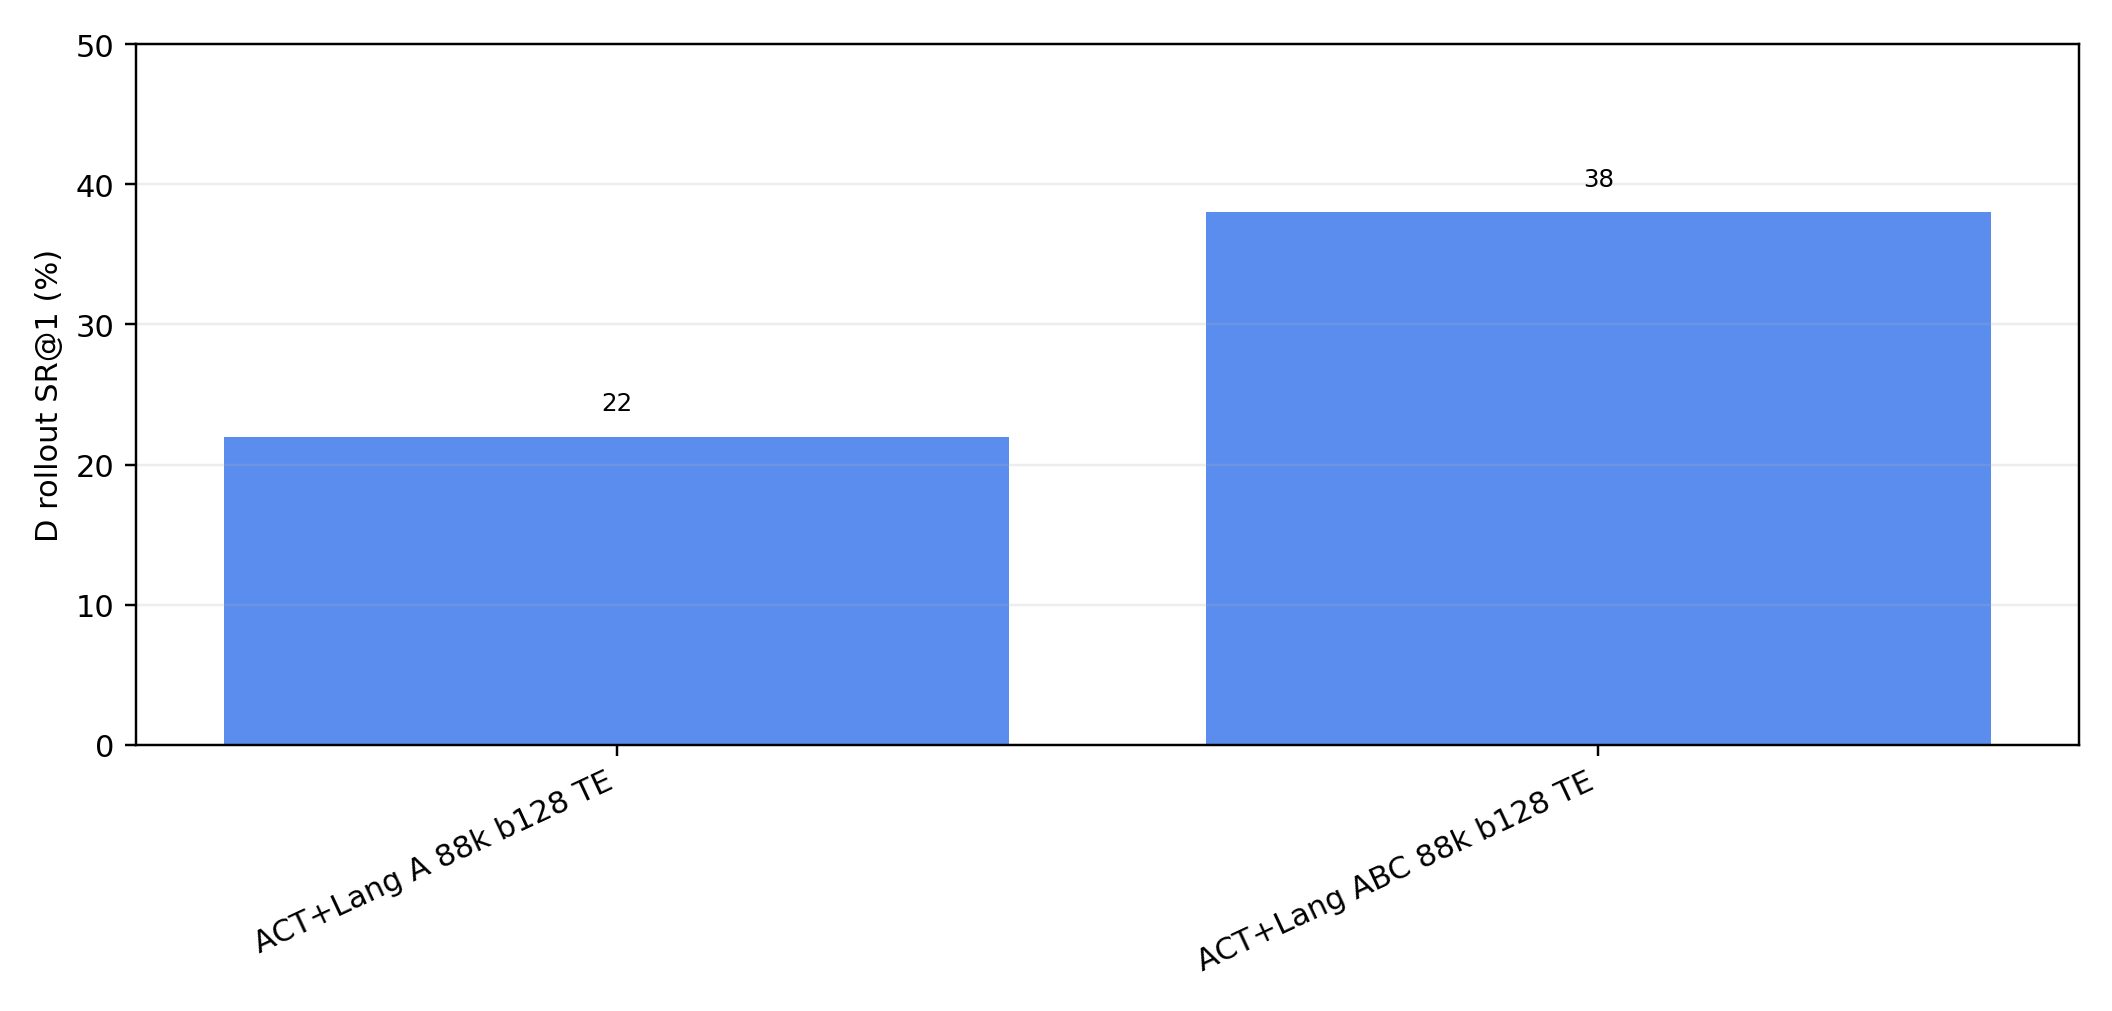
\includegraphics[width=0.95\linewidth]{figures/formal_protocol/success_rate_comparison.png}
\caption{Closed-loop SR@1 on unseen CALVIN D. The comparison is intentionally limited to the two final formal ACT policies.}
\label{fig:success}
\end{figure}

\subsection{Reading the Metric Gap}

The most useful detail is not just that ABC-joint is higher on SR@1. It is that the relative ordering flips between in-domain validation and D evaluation. If the report only used training-validation L1, A-only would look better. Once the held-out D environment is used, ABC-joint is the stronger policy. That is exactly the generalization behavior the assignment is designed to probe.

\section{Analysis}

\subsection{Why Multi-environment Training Helps}

The A-only policy can rely on stable visual features of one scene. This makes training easier but also creates a risk: some features that are predictive in A may be incidental under D. ABC-joint training exposes the encoder to more backgrounds, object appearances, and layouts. The policy is therefore pressured to represent task-relevant local geometry, gripper-object relations, and language-conditioned intent rather than a single scene's texture statistics. The held-out D results are consistent with this interpretation.

\subsection{Action Chunking Under Distribution Shift}

Action chunking helps when the observation is understood correctly. A single observation can generate a coherent short action segment, which reduces jitter and can stabilize contact timing. Under visual distribution shift, however, chunking has a second edge: a wrong interpretation can be propagated for several control steps. The chunk size of 10 is a practical compromise. It is long enough to preserve short-horizon smoothness but short enough to let new observations correct the control stream frequently.

Temporal ensembling works in the same spirit. It blends overlapping predictions to reduce abrupt action changes. In this experiment it is not credited as a separate controller, because it does not decide the task or plan the next symbolic action. It only smooths the learned ACT outputs.

\subsection{Why Offline L1 Is Not Enough}

Offline L1 compares predicted actions to demonstrations at fixed states. It is valuable for debugging because it isolates the model and preprocessing path from simulator dynamics. Closed-loop rollout is harder because the policy must live with the states it creates. A small action bias can change the next observation, which then changes the next action. This is why the report includes both metrics. The final claim is based on their agreement, not on one proxy metric alone.

\subsection{Practical Failure Modes}

The remaining errors are consistent with a lightweight behavior-cloning policy. Some failures are likely due to small object localization and gripper timing. Others are likely due to long-horizon drift after the first few actions. The final ACT policy does not include a learned high-level subtask planner, a large pretrained vision-language backbone, or multi-seed model selection. Those choices keep the experiment close to the assignment requirement, but they also limit the absolute success rate.

\section{Reproducibility}

\subsection{Artifacts}

All final artifacts are kept in the repository. The key paths are:
\begin{itemize}
  \item A-only checkpoint: \path{outputs/train/act_lang_a_only_100k_b128_v1/best}
  \item ABC checkpoint: \path{outputs/train/act_lang_abc_joint_100k_b128_v1/best}
  \item result summary: \path{reports/formal_results_summary.json}
  \item figures: \path{reports/figures/formal_protocol/}
  \item scene-D simulation snapshot: \path{reports/figures/formal_protocol/calvin_scene_d_rollout_snapshot.png}
  \item checksum file: \path{weights/SHA256SUMS.txt}
  \item upload archive: \path{dist/model_weights_act_lang_88k_b128_20260626.tar.gz}
\end{itemize}

\subsection{Environment}

The local environment used Python 3.13.5, LeRobot 0.5.2, PyTorch 2.10.0+cu128, torchvision 0.25.0+cu128, PyBullet 3.2.7, and W\&B offline logging. The GitHub-facing README includes the environment file, data preparation commands, training commands, offline evaluation commands, rollout commands, and PDF build command.

\subsection{Claim Boundaries}

The report makes one supported claim: under the fixed final ACT protocol, ABC-joint training generalizes better to D than A-only training. It does not claim leaderboard-level performance. It also does not claim that 88k is a globally optimal stopping point. The evidence is single-seed but complete for the requested comparison: both final checkpoints were trained, both were evaluated offline on D, and both were rolled out in D using the same runtime path.

\section{Conclusion}

This project completes the required LeRobot ACT comparison on CALVIN ABC$\rightarrow$D. With the same architecture and hyperparameters, the ABC-joint model outperforms the A-only model on the held-out D environment: D offline action L1 improves from 0.136686 to 0.114896, D SR@1 improves from 22\% to 38\%, and average completed subtasks improves from 0.32 to 0.56. The result shows that multi-environment ACT training improves cross-environment robustness under visual distribution shift, while the action chunking mechanism provides a useful but limited source of short-horizon stability.

\begin{thebibliography}{9}

\bibitem{mees2022calvin}
O. Mees, L. Hermann, E. Rosete-Beas, and W. Burgard.
\newblock CALVIN: A Benchmark for Language-Conditioned Policy Learning for Long-Horizon Robot Manipulation Tasks.
\newblock \emph{IEEE Robotics and Automation Letters}, 7(3):7327--7334, 2022.
\newblock doi: \href{https://doi.org/10.1109/LRA.2022.3180108}{10.1109/LRA.2022.3180108}; arXiv: \href{https://arxiv.org/abs/2112.03227}{2112.03227}.

\bibitem{zhao2023act}
T. Z. Zhao, V. Kumar, S. Levine, and C. Finn.
\newblock Learning Fine-Grained Bimanual Manipulation with Low-Cost Hardware.
\newblock In \emph{Proceedings of Robotics: Science and Systems XIX}, Daegu, Republic of Korea, July 2023.
\newblock doi: \href{https://doi.org/10.15607/RSS.2023.XIX.016}{10.15607/RSS.2023.XIX.016}.

\bibitem{lerobotact}
Hugging Face.
\newblock LeRobot Documentation: ACT (Action Chunking with Transformers).
\newblock \url{https://huggingface.co/docs/lerobot/en/act}, accessed June 26, 2026.

\bibitem{lerobotrepo}
Hugging Face.
\newblock LeRobot: Making AI for Robotics More Accessible with End-to-End Learning.
\newblock \url{https://github.com/huggingface/lerobot}, accessed June 26, 2026.

\bibitem{calvinrepo}
O. Mees, L. Hermann, E. Rosete-Beas, and W. Burgard.
\newblock CALVIN Official Repository.
\newblock \url{https://github.com/mees/calvin}, accessed June 26, 2026.

\bibitem{fywangdataset}
F. Wang.
\newblock calvin-task-ABC-D-lerobot dataset.
\newblock Hugging Face Datasets, \url{https://huggingface.co/datasets/fywang/calvin-task-ABC-D-lerobot}, accessed June 26, 2026.

\end{thebibliography}

\end{document}
